\documentclass[11pt]{standalone}

\usepackage{ifthen}
\usepackage{amsmath}
\usepackage{tikz} 
\usepackage[d]{esvect}
\usetikzlibrary{shapes.misc}
\usetikzlibrary{arrows,arrows.meta}
\usetikzlibrary{calc,intersections, patterns, math}

\definecolor{pfeil}{RGB}{168,167,167}
\definecolor{salmon}{RGB}{250,128,114}
\definecolor{petrol}{RGB}{0, 118, 136}
\definecolor{darkgoldenrod}{RGB}{184, 134, 11}
\colorlet{petrol-lighter}{petrol!40}
\colorlet{darkgoldenrod-lighter}{darkgoldenrod!40}

\begin{document}

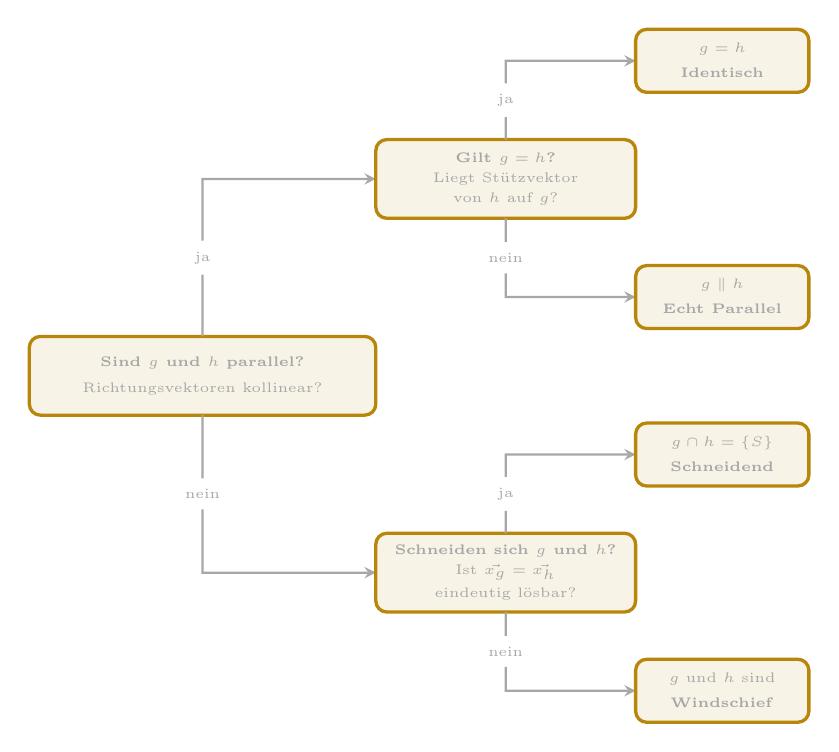
\begin{tikzpicture}[pfeil, >=stealth, very thick, xscale=1.1]
			
	% \draw[white] (-4.5,-3) rectangle (8.5,0);
			\draw[darkgoldenrod, fill=darkgoldenrod!10, rounded corners] (0,0) rectangle (4,1);
			\node at (2,0.6667) {\tiny\textbf{Sind $g$ und $h$ parallel?}};
			\node at (2,0.3333) {\tiny  Richtungsvektoren kollinear?};

			\node[rectangle] (J1) at (2,2) {\tiny ja};
			\node[rectangle] (N1) at (2,-1) {\tiny nein};
			\draw[thick,->] (2,1) -- (J1) --(2,3) -- (4,3);
			\draw[thick,->] (2,0) -- (N1) -- (2,-2) -- (4,-2);
			
			\draw[darkgoldenrod, fill=darkgoldenrod!10, rounded corners] (4,2.5) rectangle (7,3.5);
			\node at (5.5,3.25) {\tiny\textbf{Gilt $g=h$?}};
			\node at (5.5,3.) {\tiny Liegt Stützvektor};
			\node at (5.5,2.75) {\tiny  von $h$ auf $g$?};

			\node[rectangle] (J2) at (5.5,4.) {\tiny ja};
			\node[rectangle] (N2) at (5.5,2) {\tiny nein};

			\draw[thick, ->] (5.5,3.5) -- (J2) -- (5.5,4.5) -- (7,4.5);
			\draw[thick, ->] (5.5,2.5) -- (N2) -- (5.5,1.5) -- (7,1.5);
			
			\draw[darkgoldenrod, fill=darkgoldenrod!10, rounded corners] (7.,4.9) rectangle (9,4.1);
			\node at (8.,4.65) {\tiny $g=h$};
			\node at (8.,4.35) {\tiny\textbf{Identisch}};
			
			\draw[darkgoldenrod, fill=darkgoldenrod!10, rounded corners] (7.,1.9) rectangle (9,1.1);
			\node at (8.,1.65) {\tiny $g\parallel h$};
			\node at (8.,1.35) {\tiny\textbf{Echt Parallel}};
			
			% %%%%			
			\draw[darkgoldenrod, fill=darkgoldenrod!10, rounded corners] (4,-1.5) rectangle (7,-2.5);
			\node at (5.5,-1.725) {\tiny\textbf{Schneiden sich $g$ und $h$?}};
			\node at (5.5,-2.) {\tiny Ist $\vec{x_g}=\vec{x_h}$};
			\node at (5.5,-2.275) {\tiny  eindeutig lösbar?};

			\node[rectangle] (J3) at (5.5,-1) {\tiny ja};
			\node[rectangle] (N3) at (5.5,-3) {\tiny nein};

			\draw[thick, ->] (5.5,-1.5) -- (J3) -- (5.5,-0.5) -- (7,-0.5);
			\draw[thick, ->] (5.5,-2.5) -- (N3) -- (5.5,-3.5) -- (7,-3.5);
			
			\draw[darkgoldenrod, fill=darkgoldenrod!10, rounded corners] (7,-0.9) rectangle (9,-0.1);
			\node at (8,-0.35) {\tiny $g\cap h = \{S\}$};
			\node at (8,-0.65) {\tiny\textbf{Schneidend}};
			
			\draw[darkgoldenrod, fill=darkgoldenrod!10, rounded corners] (7,-3.9) rectangle (9,-3.1);
			\node at (8,-3.35) {\tiny $g$ und $h$ sind};
			\node at (8,-3.65) {\tiny\textbf{Windschief}};	

\end{tikzpicture}			

\end{document}
